\section{Work plan — Work packages, deliverables}

Brief description of the section

\subsection{Overall Structure}
%Brief presentation of the overall structure of the work plan. \textbf{Network diagram SOLO de los WP o diagrama explicativo del proyecto. El network diagram que tenemos ahora está en D2 Apartado 3.2.}

The DEOS-UD project is composed by 7 different work packages which are interrelated as shown in Figure \ref{overallstructure}. WP1 deals with project management and will ensure the proper coordination of project activities and the achievement of project objectives. WP2 is related to the quality and the administration of the project in terms of human resources, documentation management and quality, periodic monitoring and will also establish the financial plan of the project. WP3 will study the current baseline designs for the studied technologies (payload, modular system and urban development application) in the sector and will establish the potential areas of improvement and the requirements needed to achieve the new technologies proposed. WP4 is in charge of designing the output products of the project. This WP is strongly related to WP5 which is in charge of manufacturing and validating the prototype. Good intercommunication between these WPs is needed in order to obtain a final product that meets the requirements imposed by WP3. WP6 aims to create a methodology to enable the future use of the new technologies developed during the project, assuring their continuity. Finally, WP7 will ensure the project results are communicated and disseminated to the appropriate audiences, establishing new knowledge into society. 

\begin{figure}[H]
\centering
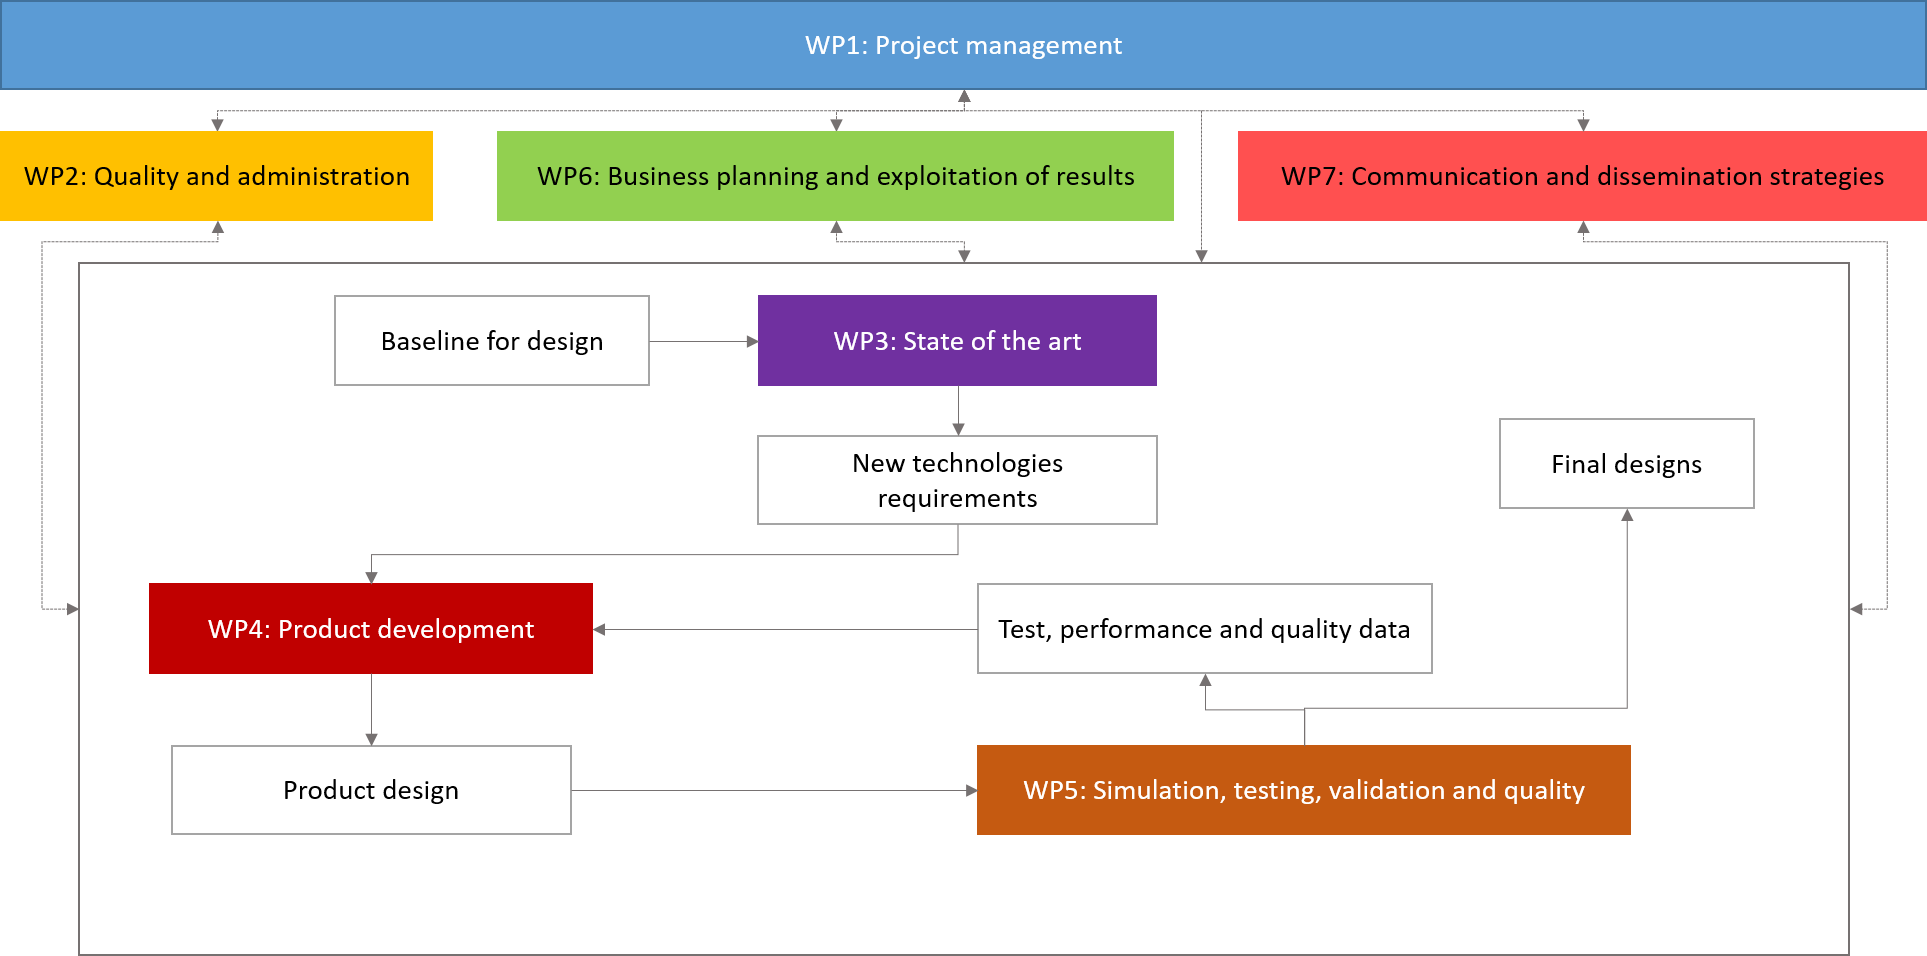
\includegraphics[width=\textwidth]{images/overallstructure.png}
\caption{DEOS-UD overall structure diagram.} 
\label{overallstructure}
\end{figure}

\subsection{Timing of the Work Plan}

Timing of the different WP: \textbf{Gantt chart. D2 Apartado 6}

\subsection{Description of Work Packages}

\begin{itemize}

\item List of WP. \textbf{D2 Apartado 2.1 Poner solo WP, no todas las activities. Extraer del D2 también Start Month i End Month}

\item Description of each WP. \textbf{Extraer información de D2 sección 2 (Número de participantes, líder, objetivos, etc.) Hay que poner las diferentes tareas dentro de cada WP y quienes participan en cada tarea. Importante: Falta calcular PM por participante. Deliverables asociados a cada WP ( también a extraer del D2).}

\end{itemize}

\begin{longtable}[H]{p{1.3cm} p{2.1cm} p{1.8cm} p{2cm} p{1.9cm} p{1.6cm} p{1.3cm}}
	\toprule[2pt]
	
	\textbf{Work Package No.} & \textbf{Work Package Title} & \textbf{Lead Participant No.} & \textbf{Lead Participant Short Name} & \textbf{Person Months} & \textbf{Start Month} & \textbf{End Month} \\
	
	\midrule[1.5pt] 
	\endhead
	
	 1& Project management & 4 & HR & 16 & M0 & M44 \vspace{0.2cm} \\
	
	\midrule

	 2& Quality and administration & 4 & HR &  26 & M0 & M44 \vspace{0.2cm} \\
	
	\midrule
	
	 3& State of the art & 1 & ADS & 34 & M1 & M3 \vspace{0.2cm} \\

	\midrule

 	 4& Product development & 1 & ADS & 119 & M4 & M29 \vspace{0.2cm} \\
 	 
 	 \midrule
 	 
 	 5& Simulation, testing, validation and quality & 7 & TAS & 27 & M22  & M43 \vspace{0.2cm} \\
 	 
 	 \midrule
 	 
 	 6& Business planning and exploitation of results & 2 & BHO & 16 & M0 & M1 \vspace{0.2cm} \\
 	 
 	 \midrule
 	 
 	 7& Communication and dissemination strategies & 4 & HR & 21 & M0 & M44 \vspace{0.2cm} \\
	
	\bottomrule[2pt]
	
	\caption{List of work packages}
	\label{workpackages}
\end{longtable}


\begin{table}[H]
\centering
\begin{tabular}{| >{\raggedright\arraybackslash}p{3cm} | >{\raggedright\arraybackslash}m{1cm} | >{\raggedright\arraybackslash}m{1cm} | >{\raggedright\arraybackslash}m{1cm}| >{\raggedright\arraybackslash}m{1cm}| >{\raggedright\arraybackslash}m{1cm} | >{\raggedright\arraybackslash}m{1cm} |>{\raggedright\arraybackslash}m{1cm}|>{\raggedright\arraybackslash}m{1cm}| }
		
		\hline
		\multicolumn{4}{|>{\raggedright\arraybackslash}l|}{\textbf{Work Package Number:}  1}&\multicolumn{5}{|>{\raggedright\arraybackslash}l|}{\textbf{Lead beneficiary:}  HIRO}\\
		
		\hline
		
		\multicolumn{9}{|>{\raggedright\arraybackslash}l|}{\textbf{Work Package Title:} Project management }\\
		
		\hline 
		
		\textbf{Participant number}&1&2&3&4&5&6&7&8\\
		
		\hline
		
		\textbf{Short name of participant}&HR&ADS&BHO&DS&IS&RSAC&TAS&VT\\
		 
		 \hline 
		 
		 \textbf{Person Month per Participant}&X&0&0&0&0&0&0&0\\
		 
		 \hline
		 
		 \multicolumn{4}{|>{\raggedright\arraybackslash}l|}{\textbf{Start Month}  M0}&\multicolumn{5}{|>{\raggedright\arraybackslash}l|}{\textbf{End month:}  M44}\\
		 
		 \hline
		
		\multicolumn{9}{|>{\raggedright\arraybackslash}l|}{\parbox[t]{14cm}{\textbf{Objectives:} \newline The aim of WP1 is to ensure a good coordination and management of the project covering technical, administrative, ethical and financial issues. The specific aims are:
\begin{itemize}
\item Coordinate DEOS-UD project providing the partners with the needed organization, supervision and leadership.
\item Manage and monitor the project progress.
\item Understand the overall project together with its risk and determination of mitigation and contingency plans for the proper development of the project.
\end{itemize}		
		}}\\
		
		\hline 
		 
		 \multicolumn{9}{|>{\raggedright\arraybackslash}l|}{\parbox[t]{14cm}{\textbf{Description of work:} \newline 
\underline{Task 1.1: Development project management plan.} \textit{Leadership: HR}. Elaboration of all the documentation that states the strategy of the management and organization of the project through its duration.\\
\underline{Task 1.2: Monitoring of the project.} \textit{Leadership: HR}. Gathering of the members of the project to inform
each other of the progress. Tracking of the active tasks and scheduling.\\
\underline{Task 1.3: Annual reporting.} \textit{Leadership: HR}. Every year that the project lasts will call for the
elaboration of an internal report with the aim of
keeping up to date with the progress done.\\
\underline{Task 1.4: Project implementation of risk management.} \textit{Leadership: HR}.Study of all the potential risks and how will they
be managed so that their affectation to the project
stays to a minimum.
		 
		 }}\\
		 \hline 
		 
		 \multicolumn{9}{|>{\raggedright\arraybackslash}l|}{\parbox[t]{14cm}{\textbf{Deliverables:} \newline \underline{Project management plan:} Document with detailed explanation
of the project management strategies,
including the Project Charter,
stakeholder register, risk, quality and
financial plans. Due date: M1}}\\
		 
		 \hline 
		 
		\end{tabular}
		
		\caption{WP1 description}
		
\end{table}


\begin{table}[H]
\begin{tabular}{| >{\raggedright\arraybackslash}p{3cm} | >{\raggedright\arraybackslash}m{1cm} | >{\raggedright\arraybackslash}m{1cm} | >{\raggedright\arraybackslash}m{1cm}| >{\raggedright\arraybackslash}m{1cm}| >{\raggedright\arraybackslash}m{1cm} | >{\raggedright\arraybackslash}m{1cm} |>{\raggedright\arraybackslash}m{1cm}|>{\raggedright\arraybackslash}m{1cm}| }
		
		\hline
		\multicolumn{4}{|>{\raggedright\arraybackslash}l|}{\textbf{Work Package Number:}  2}&\multicolumn{5}{|>{\raggedright\arraybackslash}l|}{\textbf{Lead beneficiary:}  HIRO}\\
		
		\hline
		
		\multicolumn{9}{|>{\raggedright\arraybackslash}l|}{\textbf{Work Package Title:} Quality and administration }\\
		
		\hline 
		
		\textbf{Participant number}&1&2&3&4&5&6&7&8\\
		
		\hline
		
		\textbf{Short name of participant}&ADS&BHO&DS&HR&IS&RSAC&TAS&VT\\
		 
		 \hline 
		 
		 \textbf{Person Month per Participant}&X&X&X&X&X&X&X&X\\
		 
		 \hline
		 
		 \multicolumn{4}{|>{\raggedright\arraybackslash}l|}{\textbf{Start Month}  M0}&\multicolumn{5}{|>{\raggedright\arraybackslash}l|}{\textbf{End month:}  M44}\\
		 
		 \hline
		
		\multicolumn{9}{|>{\raggedright\arraybackslash}l|}{\parbox[t]{14cm}{\textbf{Objectives:} \newline The aim of WP2 is to manage the human resources of the project in order to supply the amount of them needed to perform the project. It is also in charge of developing and controlling the financial feasibility study and seek funding to achieve the project objectives. Documentation management and periodic monitoring will also be done in this WP, assuring the quality of the deliverables and other documentation. 
		}}\\
		
		\hline 
		 
		 \multicolumn{9}{|>{\raggedright\arraybackslash}l|}{\parbox[t]{14cm}{\textbf{Description of work:} \newline 
\underline{Task 2.1: Human resources.} \textit{Leadership: HR}. Definition of the number of employees necessary and employment of them. Administration of all the employees needed to fulfill the different tasks of the project.\\
\underline{Task 2.2: Financial plan.} \textit{Leadership: HR}. Lay down of all the fix and variable costs of the project and the expected funding. Study on the economic feasibility of the project, monitoring of the evolution of the project finances and search for the additional funding for the project. \\
\underline{Task 2.3: Documentation management.} \textit{Leadership: HR}. Establishment of the guidelines for the redaction of all documents, revision of all the documents of the project and rectification of the documents that do not meet the project requirements. Approval of the reviewed and rectified documents. \\
\underline{Task 2.4: Periodic monitoring.} \textit{Leadership: HR}. To ensure the quality of the project, a periodic monitoring of all the activities will be carried out. 	 
		 }}\\
		 \hline 
		 
		 \multicolumn{9}{|>{\raggedright\arraybackslash}l|}{\parbox[t]{14cm}{\textbf{Deliverables:} \newline }}\\
		 
		 \hline 
		 
		\end{tabular}
		
		\caption{WP2 description}
		
\end{table}


\begin{table}[H]
\begin{tabular}{| >{\raggedright\arraybackslash}p{3cm} | >{\raggedright\arraybackslash}m{1cm} | >{\raggedright\arraybackslash}m{1cm} | >{\raggedright\arraybackslash}m{1cm}| >{\raggedright\arraybackslash}m{1cm}| >{\raggedright\arraybackslash}m{1cm} | >{\raggedright\arraybackslash}m{1cm} |>{\raggedright\arraybackslash}m{1cm}|>{\raggedright\arraybackslash}m{1cm}| }
		
		\hline
		\multicolumn{4}{|>{\raggedright\arraybackslash}l|}{\textbf{Work Package Number:}  3}&\multicolumn{5}{|>{\raggedright\arraybackslash}l|}{\textbf{Lead beneficiary:} \newline
		 Airbus Defence and Space}\\
		
		\hline
		
		\multicolumn{9}{|>{\raggedright\arraybackslash}l|}{\textbf{Work Package Title:} State of the art }\\
		
		\hline 
		
		\textbf{Participant number}&1&2&3&4&5&6&7&8\\
		
		\hline
		
		\textbf{Short name of participant}&ADS&BHO&DS&HR&IS&RSAC&TAS&VT\\
		 
		 \hline 
		 
		 \textbf{Person Month per Participant}&X&X&X&X&X&X&X&X\\
		 
		 \hline
		 
		 \multicolumn{4}{|>{\raggedright\arraybackslash}l|}{\textbf{Start Month}  M1}&\multicolumn{5}{|>{\raggedright\arraybackslash}l|}{\textbf{End month:}  M3}\\
		 
		 \hline
		
		\multicolumn{9}{|>{\raggedright\arraybackslash}l|}{\parbox[t]{14cm}{\textbf{Objectives:} \newline The aim of WP3 . 
		}}\\
		
		\hline 
		 
		 \multicolumn{9}{|>{\raggedright\arraybackslash}l|}{\parbox[t]{14cm}{\textbf{Description of work:} \newline 
		\underline{Task 3.1: Payloads.} \textit{Leadership: ADS. Participants: DS, TAS and HR.} Search for the current space applications and definition of the requirements for the sensors.\\
		
		\underline{Task 3.2: Modular system.} \textit{Leadership: TAS. Participants: DS, ADS and HR.} Search for the current modular systems with space applications and definition of the requirements for the modular system developed in the project.\\
		
		\underline{Task 3.3: Urban development applications with space technologies.} \textit{Leadership: IS. Participands: VT, RSAC and HR.} Search for current applications similar to those
that want to be implemented in this project in the areas of weather forecast, urban planning and greenhouse emissions reduction. Definition of the requirements of the applications.
		 }}\\
		 \hline 
		 
		 \multicolumn{9}{|>{\raggedright\arraybackslash}l|}{\parbox[t]{14cm}{\textbf{Deliverables:} \newline }}\\
		 
		 \hline 
		 
		\end{tabular}
		
		\caption{WP3 description}
		
\end{table}



\begin{table}[H]
\begin{tabular}{| >{\raggedright\arraybackslash}p{3cm} | >{\raggedright\arraybackslash}m{1cm} | >{\raggedright\arraybackslash}m{1cm} | >{\raggedright\arraybackslash}m{1cm}| >{\raggedright\arraybackslash}m{1cm}| >{\raggedright\arraybackslash}m{1cm} | >{\raggedright\arraybackslash}m{1cm} |>{\raggedright\arraybackslash}m{1cm}|>{\raggedright\arraybackslash}m{1cm}| }
		
		\hline
		\multicolumn{4}{|>{\raggedright\arraybackslash}l|}{\textbf{Work Package Number:}  4}&\multicolumn{5}{|>{\raggedright\arraybackslash}l|}{\textbf{Lead beneficiary:} \newline
		 Airbus Defence and Space}\\
		
		\hline
		
		\multicolumn{9}{|>{\raggedright\arraybackslash}l|}{\textbf{Work Package Title:} Product development }\\
		
		\hline 
		
		\textbf{Participant number}&1&2&3&4&5&6&7&8\\
		
		\hline
		
		\textbf{Short name of participant}&ADS&BHO&DS&HR&IS&RSAC&TAS&VT\\
		 
		 \hline 
		 
		 \textbf{Person Month per Participant}&X&X&X&X&X&X&X&X\\
		 
		 \hline
		 
		 \multicolumn{4}{|>{\raggedright\arraybackslash}l|}{\textbf{Start Month}  M4}&\multicolumn{5}{|>{\raggedright\arraybackslash}l|}{\textbf{End month:}  M29}\\
		 
		 \hline
		
		\multicolumn{9}{|>{\raggedright\arraybackslash}l|}{\parbox[t]{14cm}{\textbf{Objectives:} \newline The aim of WP4 . 
		}}\\
		
		\hline 
		 
		 \multicolumn{9}{|>{\raggedright\arraybackslash}l|}{\parbox[t]{14cm}{\textbf{Description of work:} \newline 
		\underline{Task 4.1: Preliminary design.} \textit{Leadership: ADS. Participants: DS, TAS, HR, VT, RSAC, IS}. Research for the payload preliminary design and development of it. Modular system preliminary design, definition of SATCOM application domains and development of: physical framework for sensor block, systems interactions and applications, sensor data fusion software. Preliminary design of the interaction platform and implementation of web-based servers for sharing sensors data and processing algorithms based on applications.\\
		 
		\underline{Task 4.2: Final design:} \textit{Leadership: ADS. Participants: DS, TAS, HR, VT, RSAC, IS}. Final design and technical specifications of the payload sensors. Final design of the modular system, specifically the sensors data fusion software. Final design and implementation of the interaction platform, including the web servers for data sharing and the processing algorithms. 
		
		 }}\\
		 \hline 
		 
		 \multicolumn{9}{|>{\raggedright\arraybackslash}l|}{\parbox[t]{14cm}{\textbf{Deliverables:} \newline }}\\
		 
		 \hline 
		 
		\end{tabular}
		
		\caption{WP4 description}
		
\end{table}

\subsection{Deliverables}

List of deliverables and milstones. \textbf{D2 sección 1.2}

KEY: Deliverable numbers in order of delivery dates. Please use the numbering convention <WP number>.<number of deliverable within that WP>.

For example, deliverable 4.2 would be the second deliverable from work package 4.

Type: Use one of the following codes:
\begin{itemize}
\item R: Document, report (excluding the periodic and final reports) 
\item DEM: Demonstrator, pilot, prototype, plan designs
\item DEC: Websites, patents filing, press i media actions, videos, etc. 
\item OTHER: Software, technical diagram, etc.
\end{itemize}

Dissemination level: Use one of the following codes:
\begin{itemize}
\item PU = Public, fully open, e.g. web
\item CO = Confidential, restricted under conditions set out in Model Grant Agreement
\item CI = Classified, information as referred to in Commission Decision 2001/844/EC.
\end{itemize}

Deliverable Date: Measured in months from the project start date (month 1)

\begin{longtable}[H]{p{1.8cm} p{2cm} p{1.3cm} p{1.8cm} p{1.3cm} p{2.1cm} p{1.8cm}}
	\toprule[2pt]
	
	\textbf{Deliverable No.} & \textbf{Deliverable Name} & \textbf{Work Package No.} & \textbf{Lead Participant Short Name} & \textbf{Type} & \textbf{Disemination Level} & \textbf{Deliverable Date} \\
	
	\midrule[1.5pt] 
	\endhead
	
	&  &  &  &  &  & \vspace{0.2cm} \\
	
	\midrule

	 &  &  &  &  &  & \vspace{0.2cm} \\
	
	\midrule
	
	 &  &  &  &  &  &  \vspace{0.2cm} \\

	\midrule

 	 &  &  &  &  &  &  \vspace{0.2cm} \\
	
	\bottomrule[2pt]
	
	\caption{List of Deliverables}
	\label{workpackages}
\end{longtable}


\subsection{Inter-relation between components}

Graphical presentation of the components showing how they inter-relate (Per chart or similar) \textbf{Algo más sencillo que el network diagram. Podría ser el network diagram.}


